%!TEX program = xelatex
\documentclass[cn,hazy,blue,14pt,screen]{elegantnote}
\title{Ptolemy:平衡机器算法应用运行辅助工具}

\author{施华}
\institute{Algorithm application operation assistant tool}

\version{beta-0.1}
\date{\zhtoday}

\usepackage{array}

\begin{document}

\maketitle

\centerline{
  \includegraphics[width=0.2\textwidth]{logo-ae.png}
}



\section{Ptolemy介绍}

Ptolemy是一个算法应用运行管理辅助工具,目前主要提供算法结果收集与算法作业的监控工作。

Ptolemy有下面几个特性:

\begin{itemize}
  \item 高度自由化,可自定义
  \item 基于时序数据库存储信息,高性能。
\end{itemize}

以下主要是主体框架和基础套餐的设计说明



\subsection{主体框架}

Ptolemy充分利用Python动态语言特性,基于InfluxDB时序数据库的数据结构和高性能,封装了读写数据API和对象映射模型。主要涉及的技术有:

\begin{enumerate}[label=\arabic*).]
	\item \textit{InfluxDB}\\
	主要利用时序数据库的数据结构来存储算法应用作业和结果信息,读写速度快于常用数据库100到1000倍。
	\item \textit{ORM}\\
	主要利用type和构建技术基础方法,构建了InfluxDB的ORM模型,方便自由开发使用。
\end{enumerate}

\centerline{
	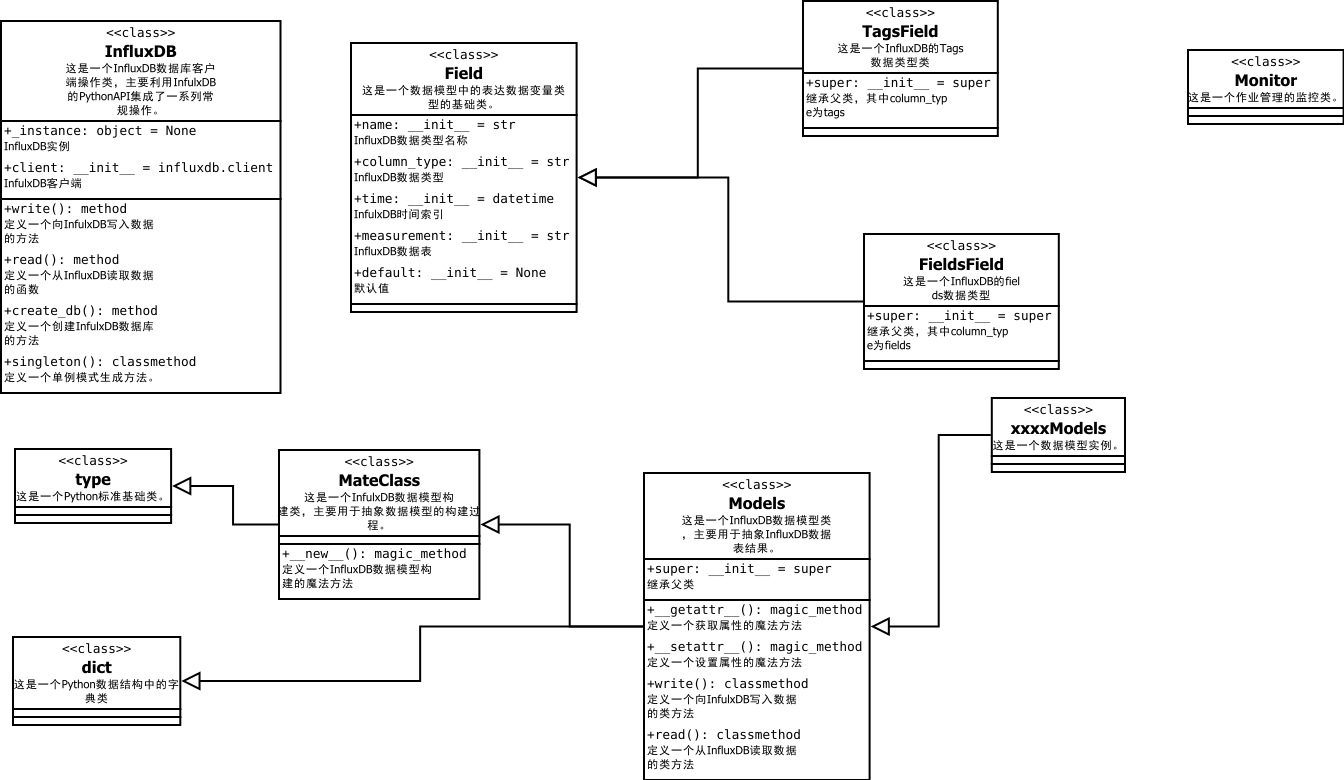
\includegraphics[width=0.8\textwidth]{Ptolemy.png}
}








\subsection{使用示例}

Ptolemy的API可分为两级,第一级主要是InfluxDB的读写数据操作封装,第二级主要是一个基于InfluxDB的对象映射模型。

代码示例:

\begin{lstlisting}
	from Ptolemy.influxdb_base import *
	from Ptolemy.orm import *
	import pandas as pd 
	
	'10.2.12.248', 8086, 'test', 'test', 'example'
	
	host = '10.2.12.248'
	port = 8086
	user = 'test'
	password = 'test'
	database = 'example'
	method = 'JSON'
	
	
	############# JSON Client #########################################
	### 连接数据库
	InfluxDB_JSON = InfluxDB(host,port,user,password,database,method)
	InfluxDB_Client = InfluxDB_JSON.get_client()
	### 列出数据库
	db_list = InfluxDB_Client.get_list_database()
	print(db_list)
	### 写入数据
	json_body = [
	{
		"measurement": "cpu_load_short",
		"tags": {
			"host": "server04",
			"region": "us-west"
		},
		"time": "2009-11-10T23:00:00Z",
		"fields": {
			"value": 0.99
		}
	}
	]
	write_result = InfluxDB_JSON.write_json(json_body)
	print(write_result)
	### 查询数据
	query = 'select * from cpu_load_short'
	query_result = InfluxDB_JSON.read_json(query = query)
	print(query_result)
	
	####### 一级API ##################################################
	##################################################################
	
	
	
	############# DataFrame Client ####################################
	host = '10.2.12.248'
	port = 8086
	user = 'test'
	password = 'test'
	database = 'example1'
	method = 'DataFrame'
	protocol = 'line'
	### 连接数据库
	InfluxDB_DataFrame = InfluxDB(host,port,user,password,database,method)
	InfluxDB_Client = InfluxDB_DataFrame.get_client()
	### 列出数据库
	db_list = InfluxDB_Client.get_list_database()
	print(db_list)
	df = pd.DataFrame(data=list(range(30)),
	index=pd.date_range(start='2014-11-16',
	periods=30, freq='H'), columns=['0'])
	# ### 写入带标签的DataFrame
	# InfluxDB_DataFrame.write_dataframe(df,'demo',
	#                     {'k1': 'v1', 'k2': 'v2'},'line')
	### 查询数据
	tmp_query = InfluxDB_DataFrame.read_dataframe("select * from demo")
	print(tmp_query)
	### 统一查询接口
	tmp_1 = InfluxDB_DataFrame.query('select * from demo')
	tmp_2 = InfluxDB_JSON.query('select * from cpu_load_short where value = 0.99')
	print("------------------------------------------------------")
	points_1 = tmp_1.get_points()
	for i in points_1:
	print(i)
	print("------------------------------------------------------")
	points_2 = tmp_2.get_points()
	print(tmp_2)
	
	
	
	#### 二级API ############################################################
	#########################################################################
	
	
	### 构建数据模型基础类
	class cpu_load_short(Models):
	value = FieldsField(name = 'value',tag_key = False)
	host = TagsField(name = 'host',tag_key = True)
	region = TagsField(name = 'region',tag_key = True)
	
	
	import pandas as pd 
	df = pd.DataFrame(data=list(range(30)),
	index=pd.date_range(start='2014-11-16',
	periods=30, freq='H'), columns=['0'])
	
	
	class demo(Models):
	dataframe = df
	tag_dict = {'k1': 'v1', 'k2': 'v2'}
	
	
	
	
	### 构建数据模型
	cpu_load_short = cpu_load_short(value = 1.11,host = 'server05',region = 'us-test')
	demo = demo()
	### 连接InfluxDB数据库
	host = '10.2.12.248'
	port = 8086
	user = 'test'
	password = 'test'
	database = 'example'
	method = 'JSON'
	InfluxDB_JSON = InfluxDB(host,port,user,password,database,method)
	host = '10.2.12.248'
	port = 8086
	user = 'test'
	password = 'test'
	database = 'example1'
	method = 'DataFrame'
	protocol = 'line'
	InfluxDB_DataFrame = InfluxDB(host,port,user,password,database,method)
	### 保存数据模型种的数据
	write_result_1= cpu_load_short.save_json(influxdb_obj = InfluxDB_JSON,save_time = '2009-11-10T23:00:00Z')
	write_result_2 = demo.save_dataframe(influxdb_obj = InfluxDB_DataFrame)
	print(write_result_1)
	print(write_result_2)
	### 查询数据结构表
	query_result_1 = cpu_load_short.query(influxdb_obj = InfluxDB_JSON)
	query_result_2 = demo.query(InfluxDB_DataFrame)
	points_1 = query_result_1.get_points()
	points_2 = query_result_2.get_points()
	for i in points_1:
	print(i)
	for j in points_2:
	print(j)
\end{lstlisting}



\end{document}
